\chapter{Chinchilla — compute-optimal training}
\label{ch:chinchilla}

\newthought{Two years after Kaplan,} a team at DeepMind \citep{hoffmann2022training}
ran a wider sweep over model size \(N\) and data \(D\), trained each
configuration to convergence, and asked a sharper question. Given a fixed
training compute budget \(C\), what is the best joint choice of
\((N, D)\)?

\section{The isoflops surface}

Compute, parameters, and tokens are tied by a simple rule of thumb:
\begin{equation}
  C \;\approx\; 6 \cdot N \cdot D
  \label{eq:flops}
\end{equation}
FLOPs to train a transformer with \(N\) parameters on \(D\)
tokens.\sidenote{The factor of 6 is bookkeeping. Forward pass is roughly
\(2 N D\) FLOPs; backward pass is twice that; the constant absorbs ``per
token, per parameter''. \citet{kaplan2020scaling} discuss this carefully.}

So an \emph{isoflops curve} (constant \(C\)) is a hyperbola \(N \cdot D =
\text{const}\) in the \((N, D)\) plane. Along this curve, you can buy a
bigger model by training it on less data, or vice versa. The Chinchilla
question is: where on the curve is the loss lowest?

\begin{figure}
\centering
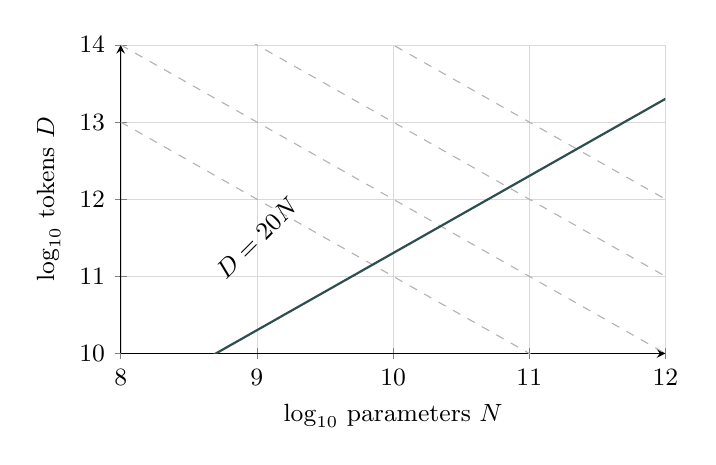
\begin{tikzpicture}
\begin{axis}[
  width=8.5cm, height=5.5cm,
  xlabel={\(\log_{10}\) parameters \(N\)},
  ylabel={\(\log_{10}\) tokens \(D\)},
  xmin=8, xmax=12, ymin=10, ymax=14,
  axis lines=left,
  grid=both,
  major grid style={line width=.1pt, draw=gray!30},
  tick pos=left,
  ticklabel style={font=\small},
  label style={font=\small},
]
  % Isoflops contours: log10(N) + log10(D) = const
  \foreach \k in {21,22,23,24} {
    \addplot[domain=8:12, samples=2, dashed, color=gray!60]
      {\k - x};
  }
  % Optimal line: D = 20 N => log10(D) = log10(N) + log10(20)
  \addplot[domain=8:12, samples=2, thick, color=DarkSlateGray]
    {x + 1.301};
  \node[font=\small, rotate=45] at (axis cs:9.0,11.5) {\(D = 20 N\)};
\end{axis}
\end{tikzpicture}
\caption{Schematic of the Chinchilla finding. Dashed grey lines are
isoflops contours (\(N \cdot D\) constant). The thick line through the
optimum sits at roughly \(D = 20 N\): for every billion parameters, train
on about 20 billion tokens.}
\end{figure}

\section{The 20:1 rule}

The empirical optimum sits along
\begin{equation}
  D \;\approx\; 20 \cdot N
\end{equation}
for a wide range of compute budgets. Concretely:

\begin{center}
\begin{tabular}{lll}
\toprule
Model & Params & Tokens \\
\midrule
GPT-3 (Kaplan-pilled) & 175B & ${\sim}300$B \\
Chinchilla            & 70B  & ${\sim}1.4$T \\
Llama 1 (7B)          & 7B   & 1T \\
Llama 2 (7B)          & 7B   & 2T \\
Llama 3 (8B)          & 8B   & 15T \\
\bottomrule
\end{tabular}
\end{center}

The empirical pattern from 2022 onward has been to push the
token-to-parameter ratio \emph{above} 20, because at inference time a
smaller model is cheaper to serve. Llama 3's 15T tokens per 8B parameters
(${\sim}1900{:}1$) reflects that bias: take the loss hit on training
efficiency to get a deployment-friendly model.\sidenote{This is sometimes
called ``inference-Chinchilla''. If you plan to serve the model to billions
of requests, the right cost function isn't training compute — it is
training compute plus the integral of inference cost over the model's
lifetime. That argues strongly for over-training a smaller model.}

\section{The headline result}

The dramatic single experiment in the Chinchilla paper: a 70B model trained
on 1.4T tokens \emph{beat} a 280B model (Gopher) trained on 300B tokens, on
the same total compute budget. Smaller, more data, better.

This rewrote the recipe for every frontier lab in 2022--2023. Llama,
Mistral, Gemma, Mixtral, Qwen, Phi — every public model since reflects this
correction in some form.

\section{Bridge to long context}

Both Kaplan and Chinchilla say that loss is a smooth function of \emph{train-time}
resources. They are completely silent on \emph{inference-time} cost — and
specifically silent on the question we have been building toward: how much
does it cost to \emph{use} a context of length \(n\)?

That silence is intentional. The training-loss-versus-resources story holds
even with very short contexts; you do not need a 1M-token context window to
fit a power law. But the moment you ask the model to actually read a long
document at inference time, the costs from Chapter~\ref{ch:why-quadratic}
hit, and they are not in the scaling laws at all.

That gap is what Chapter~\ref{ch:what-scaling-omits} is about, and what
the rest of this book is fundamentally a response to.

\keyidea{Chinchilla says training compute is best spent on smaller models
fed more tokens than Kaplan recommended. It does not say anything about
how to spend inference compute on long contexts. The latter is the entire
problem this book exists to discuss.}
